% 第2章第5节：算子的伴随与空间分解（伴随算子、像与核、自伴与正算子及正交投影、条件期望的投影解释）。

\section{算子的伴随与空间分解}
\label{sec:lfo-adjoint}

本节回到Hilbert空间之间的一般算子。前两节说明，Hilbert空间中的每个连续读数都是一个方向；现在用这一点研究算子怎样把输出空间中的测试方向对应回输入空间，并由此回答两个问题：哪些输入方向在输出中完全看不见，哪些输出能被算子的像逼近。自伴与正性进一步刻画同一空间中的方向关系，正交投影和条件期望是最重要的例子。

\subsection{伴随算子}
\label{sec:lfo-adjoint-def}

\paragraph{把输出测试拉回输入}
设$H_1,H_2$是Hilbert空间，$A\in\mathcal B(H_1,H_2)$。固定输出空间中的方向$v\in H_2$，考察读数$u\mapsto\langle v,Au\rangle$：先把输入$u$送到输出空间，再用$v$去测试。它对$u$线性，且$|\langle v,Au\rangle|\leq\|v\|\,\|A\|\,\|u\|$，所以是$H_1$上的有界线性泛函。由Riesz表示定理，存在唯一的$w\in H_1$使$\langle v,Au\rangle=\langle w,u\rangle$对一切$u$成立。这个$w$随$v$而定，记为$A^*v$。

\begin{definition}[伴随算子]
\label{def:lfo-adjoint}
设$A\in\mathcal B(H_1,H_2)$。由
\begin{equation}
 \langle v,Au\rangle_{H_2}=\langle A^*v,u\rangle_{H_1}\qquad(u\in H_1,\ v\in H_2)
 \label{eq:lfo-adjoint}
\end{equation}
确定的映射$A^*:H_2\to H_1$称为$A$的\term{伴随}（adjoint）算子。
\end{definition}

伴随回答的问题是：用输出方向$v$测试$Au$，相当于在输入空间中用哪个方向测试$u$。它把测试方向从输出空间拉回输入空间，并不是从输出恢复输入。下面的移位算子会清楚地显示这一区别。

\begin{theorem}[伴随的基本性质]
\label{thm:lfo-adjoint-properties}
设$A,B\in\mathcal B(H_1,H_2)$，$C\in\mathcal B(H_2,H_3)$，$\alpha\in\mathbb F$。则$A^*\in\mathcal B(H_2,H_1)$，并且
\[
 \begin{aligned}
 &(A+B)^*=A^*+B^*,\quad(\alpha A)^*=\bar\alpha A^*,\quad(CA)^*=A^*C^*,\\
 &A^{**}=A,\quad\|A^*\|=\|A\|,\quad\|A^*A\|=\|A\|^2 .
 \end{aligned}
\]
\end{theorem}

\begin{proof}
\emph{线性。}对$v_1,v_2$及标量$\beta_1,\beta_2$，$\langle A^*(\beta_1v_1+\beta_2v_2),u\rangle=\langle\beta_1v_1+\beta_2v_2,Au\rangle=\bar\beta_1\langle A^*v_1,u\rangle+\bar\beta_2\langle A^*v_2,u\rangle=\langle\beta_1A^*v_1+\beta_2A^*v_2,u\rangle$，由Riesz表示的唯一性即得。和、数乘与复合的公式用同样的方式验证，例如$\langle v,CAu\rangle=\langle C^*v,Au\rangle=\langle A^*C^*v,u\rangle$；数乘中的共轭来自内积对第一个变量共轭线性。

\emph{有界与范数。}由$\|A^*v\|^2=\langle A^*v,A^*v\rangle=\langle v,AA^*v\rangle\leq\|v\|\,\|A\|\,\|A^*v\|$得$\|A^*v\|\leq\|A\|\,\|v\|$，即$\|A^*\|\leq\|A\|$。对$A^*$的伴随求共轭可知$\langle u,A^*v\rangle=\langle Au,v\rangle$，所以$A^{**}=A$，再用一次刚才的不等式得$\|A\|=\|A^{**}\|\leq\|A^*\|$。

\emph{$\|A^*A\|=\|A\|^2$。}一方面$\|A^*A\|\leq\|A^*\|\,\|A\|=\|A\|^2$；另一方面对单位向量$u$，$\|Au\|^2=\langle u,A^*Au\rangle\leq\|A^*A\|$，取上确界得$\|A\|^2\leq\|A^*A\|$。
\end{proof}

\paragraph{矩阵与积分核}
在$\mathbb F^n$与$\mathbb F^m$上配标准内积，矩阵$\bm A$的伴随就是共轭转置$\bm A^{\mathsf H}$，实情形即转置。函数空间中，最常见的例子是积分算子。在$L^2(0,1)$上取$(Vu)(s)=\int_0^su(t)\,dt$，即从$0$累积到$s$。对$v\in L^2(0,1)$，由Fubini定理（定理~\ref{thm:integral-fubini}，被积函数在三角形区域上可积）交换积分次序：
\[
 \langle v,Vu\rangle=\int_0^1\overline{v(s)}\int_0^su(t)\,dt\,ds=\int_0^1\Bigl(\int_t^1\overline{v(s)}\,ds\Bigr)u(t)\,dt ,
\]
所以$(V^*v)(t)=\int_t^1v(s)\,ds$，即从$t$累积到$1$。用$u=v=1$核对：$\langle1,V1\rangle=\int_0^1s\,ds=1/2$，$V^*1=1-t$，$\langle V^*1,1\rangle=\int_0^1(1-t)\,dt=1/2$。一般地，核为$k(s,t)$的积分算子，其伴随的核是$\overline{k(t,s)}$，第~\ref{sec:ose-kernel-symmetry}节将系统讨论。

\paragraph{伴随不是逆}
在$\ell^2$上，右移$S(x_1,x_2,\ldots)=(0,x_1,x_2,\ldots)$的伴随是左移$S^*(y_1,y_2,\ldots)=(y_2,y_3,\ldots)$：逐项核对$\langle y,Sx\rangle=\sum_{k\geq1}\bar y_{k+1}x_k=\langle S^*y,x\rangle$。于是$S^*S=I$，左移撤销了右移；但$SS^*(y_1,y_2,\ldots)=(0,y_2,y_3,\ldots)$，第一个坐标被抹掉了，$SS^*\neq I$。$S$保持长度，不丢失信息，但它的像缺少$e_1$方向，所以$S^*$只是左逆。对一般算子，$A^*$连左逆都不是：零算子的伴随是零算子。

\paragraph{Banach空间中的转置}
没有内积时，仍然可以把输出读数拉回输入。对$A\in\mathcal B(X,Y)$，令$A'L=L\circ A$，$L\in Y^*$，得到\term{转置算子}（transpose operator）$A':Y^*\to X^*$。由定理~\ref{thm:lfo-norming-functional}可以证明$\|A'\|=\|A\|$。转置作用在对偶空间之间；只有在Hilbert空间中借助Riesz对应把读数换成向量，才能把它写成作用在$H_2$与$H_1$之间的伴随$A^*$。

\subsection{像空间与零空间}
\label{sec:lfo-range-kernel}

\paragraph{正交关系}
伴随的定义式~\eqref{eq:lfo-adjoint}把“输出与$Au$正交”翻译成输入空间中的条件。记$\operatorname{Ran}A=\{Au:u\in H_1\}$为像，$\ker A=\{u:Au=0\}$为核。

\begin{theorem}[像与核的正交关系]
\label{thm:lfo-range-kernel}
设$A\in\mathcal B(H_1,H_2)$。则
\begin{equation}
 (\operatorname{Ran}A)^\perp=\ker A^*,\qquad\overline{\operatorname{Ran}A}=(\ker A^*)^\perp ,
 \label{eq:lfo-range-kernel}
\end{equation}
交换$A$与$A^*$的角色，又有$(\operatorname{Ran}A^*)^\perp=\ker A$与$\overline{\operatorname{Ran}A^*}=(\ker A)^\perp$。
\end{theorem}

\begin{proof}
$y\in(\operatorname{Ran}A)^\perp$，当且仅当对一切$u$有$\langle y,Au\rangle=0$，即$\langle A^*y,u\rangle=0$；取$u=A^*y$可知这等价于$A^*y=0$。这证明了第一个等式。

对第二个等式，只需说明线性子空间$M$满足$(M^\perp)^\perp=\overline M$，再取$M=\operatorname{Ran}A$。显然$M\subset(M^\perp)^\perp$，后者是闭集，所以$\overline M\subset(M^\perp)^\perp$。反过来，设$y\in(M^\perp)^\perp$，由第~\ref{sec:fs-projection}节的正交分解$y=P_{\overline M}y+z$，$z\in(\overline M)^\perp=M^\perp$；而$y$与$P_{\overline M}y$都与$z$正交，所以$\|z\|^2=\langle z,y-P_{\overline M}y\rangle=0$，$y\in\overline M$。其余两式把$A$换成$A^*$并用$A^{**}=A$即得。
\end{proof}

由此得到两个空间的正交分解：
\[
 H_1=\ker A\oplus\overline{\operatorname{Ran}A^*},\qquad H_2=\ker A^*\oplus\overline{\operatorname{Ran}A} .
\]
图~\ref{fig:lfo-four-subspaces}把这四个子空间放在一起。$\ker A$中的输入方向在输出中完全看不见，加到任何输入上都不改变输出；$\overline{\operatorname{Ran}A}$是能被输出逼近的方向；$\ker A^*$中的输出方向与一切输出正交，任何输入都到达不了。这是有限维中“四个基本子空间”在Hilbert空间中的形式，区别在于像必须取闭包。

\begin{figure}[!htb]
  \centering
  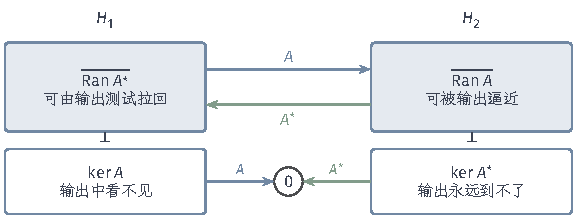
\includegraphics[width=97.7mm]{figures/02-abstract-mathematics/03-function-spaces/tikz/c2-four-subspaces/figure.pdf}
  \caption{伴随与像、核的正交关系。输入空间分解为$H_1=\ker A\oplus\overline{\operatorname{Ran}A^*}$，输出空间分解为$H_2=\ker A^*\oplus\overline{\operatorname{Ran}A}$。$A$把$\ker A$送到零，其余输入的输出都落在$\operatorname{Ran}A$中；$A^*$把$\ker A^*$送到零。无限维中像未必闭合，正交关系只确定像的闭包。}
  \label{fig:lfo-four-subspaces}
\end{figure}

\paragraph{累积算子的像}
以上面的$V$为例。若$V^*v=0$，则$\int_t^1v(s)\,ds=0$对一切$t$成立，于是$v$在每个区间$(t,1)$上积分为零，从而$v=0$几乎处处，$\ker V^*=\{0\}$。由式~\eqref{eq:lfo-range-kernel}，$\operatorname{Ran}V$在$L^2(0,1)$中稠密。但$\operatorname{Ran}V$中的函数都是连续的，阶跃函数$\mathbf 1_{(1/2,1)}$不在其中，所以$\operatorname{Ran}V\neq L^2(0,1)$：像稠密而不闭。

\paragraph{像稠密不闭的数列例子}
在$\ell^2$上令$A(x_n)=(x_n/n)$，即第$n$个坐标乘以$1/n$。它是自伴的（$A^*=A$），单射，所以$\ker A^*=\{0\}$，像在$\ell^2$中稠密。考察$y=(1/n)$，由$\sum_n1/n^2<\infty$知$y\in\ell^2$。若$Ax=y$，逐个坐标比较得$x_n=1$，这个唯一的形式逆像不是平方可和的，所以$y\notin\operatorname{Ran}A$。

截断形式逆像可以看清发生了什么。令$x^{(N)}=(1,\ldots,1,0,0,\ldots)$，前$N$个坐标为$1$。则
\[
 \|Ax^{(N)}-y\|^2=\sum_{n>N}\frac1{n^2}\longrightarrow0,\qquad\|x^{(N)}\|=\sqrt N\longrightarrow\infty .
\]
图~\ref{fig:lfo-dense-range}显示：残差随$N$增大趋于零，说明$y$在像的闭包中；为了取得这些越来越好的近似，输入的范数却无限增大。输出上越来越小的修正需要越来越大的输入，这正是第~\ref{sec:lfo-inverse}节要讨论的不稳定性。

\begin{figure}[!htb]
  \centering
  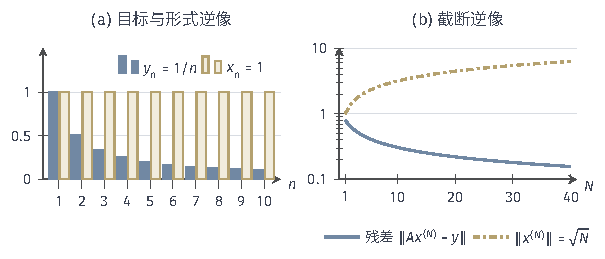
\includegraphics[width=102.5mm]{figures/02-abstract-mathematics/03-function-spaces/tikz/c2-dense-range/figure.pdf}
  \caption{$\ell^2$上$A(x_n)=(x_n/n)$的像稠密而不闭。(a)~目标$y_n=1/n$（蓝）平方可和，但唯一的形式逆像$x_n=1$（黄）不平方可和；(b)~截断逆像$x^{(N)}$的残差$\|Ax^{(N)}-y\|$（蓝）趋于零，范数$\|x^{(N)}\|=\sqrt N$（黄点划线）趋于无穷，纵轴为对数刻度。}
  \label{fig:lfo-dense-range}
\end{figure}

\paragraph{正交条件只确定像的闭包}
这个例子划出了正交关系的边界。$y\perp\ker A^*$只能保证$y$在像的闭包中，不能保证方程$Ax=y$精确可解。只有已经知道$\operatorname{Ran}A$闭合时，才有$\operatorname{Ran}A=(\ker A^*)^\perp$，此时$Ax=y$可解当且仅当$y$与$\ker A^*$正交。第~\ref{chap:operator-spectra-equations}章的Fredholm理论和第一类方程都会反复使用这一边界。

\subsection{自伴、正算子与正交投影}
\label{sec:lfo-self-adjoint}

\paragraph{自伴与正算子}
当输入和输出在同一个Hilbert空间$H$中时，可以比较$A$与$A^*$。若$A=A^*$，即$\langle v,Au\rangle=\langle Av,u\rangle$对一切$u,v$成立，则称$A$为\term{自伴}（self-adjoint）算子。自伴算子的二次型$\langle x,Ax\rangle$总是实数，因为它等于自身的共轭$\langle Ax,x\rangle$。

\begin{definition}[正算子]
\label{def:lfo-positive-operator}
设$A\in\mathcal B(H)$自伴。若$\langle x,Ax\rangle\geq0$对一切$x\in H$成立，则称$A$为\term{正算子}（positive operator），记为$A\geq0$。
\end{definition}

定义中要求先自伴，是因为在实空间中二次型非负并不能推出对称：平面上逆时针旋转$90^\circ$的矩阵满足$\bm x^{\top}\bm A\bm x=0$，却不对称。最基本的正算子是$A^*A$：$\langle x,A^*Ax\rangle=\|Ax\|^2\geq0$。

\paragraph{三种强度的正性}
对自伴算子，下面三个条件依次加强：（i）$\langle x,Ax\rangle\geq0$对一切$x$成立；（ii）$\langle x,Ax\rangle>0$对一切$x\neq0$成立；（iii）存在常数$c>0$，使$\langle x,Ax\rangle\geq c\|x\|^2$对一切$x$成立，此时称$A$具有\term{强制性}（coercivity）。有限维中（ii）与（iii）等价，因为单位球面紧，连续函数在其上取到正的最小值；无限维中不再如此。上一小节的$A(x_n)=(x_n/n)$满足（ii），因为$\langle x,Ax\rangle=\sum_n|x_n|^2/n>0$；但$\langle e_n,Ae_n\rangle=1/n\to0$，没有统一的下界$c$。逐方向严格为正，不能当作统一下界。

统一下界对逆向恢复有直接意义。若$A$自伴且强制，则由Cauchy--Schwarz不等式$c\|x\|^2\leq\langle x,Ax\rangle\leq\|x\|\,\|Ax\|$，得$\|Ax\|\geq c\|x\|$。由此$A$单射；像是闭的，因为若$Ax_n\to y$，则$\|x_n-x_m\|\leq c^{-1}\|Ax_n-Ax_m\|$，$(x_n)$是Cauchy列，极限$x$满足$Ax=y$；又$\ker A^*=\ker A=\{0\}$，由定理~\ref{thm:lfo-range-kernel}像稠密。像既闭又稠密，所以$A$是双射，且$\|A^{-1}\|\leq1/c$。只有逐方向严格正的算子则可能像不闭，正如$(x_n/n)$。

\paragraph{正交投影的算子刻画}
第~\ref{sec:fs-projection}节从最近点问题得到了正交投影$P_M$。现在用算子性质刻画它。

\begin{theorem}[正交投影的刻画]
\label{thm:lfo-orthogonal-projection}
设$P\in\mathcal B(H)$。则$P$是到某个闭子空间的正交投影，当且仅当$P^2=P$且$P^*=P$。此时该子空间为$M=\operatorname{Ran}P$，且$P\geq0$，$\|P\|\leq1$。
\end{theorem}

\begin{proof}
若$P=P_M$，则$P^2=P$是因为$M$中元素的投影是它自己。对任意$x,z$，$\langle z,Px\rangle=\langle Pz+(z-Pz),Px\rangle=\langle Pz,Px\rangle$，因为$z-Pz\perp M$；同理$\langle Pz,x\rangle=\langle Pz,Px\rangle$，所以$P^*=P$。

反过来，设$P^2=P=P^*$。令$M=\operatorname{Ran}P$。由$P^2=P$，$M=\ker(I-P)$，是闭子空间。对任意$x$，$Px\in M$，而$x-Px\in\ker P$；由定理~\ref{thm:lfo-range-kernel}，$\ker P=\ker P^*=(\operatorname{Ran}P)^\perp=M^\perp$。所以$x=Px+(x-Px)$恰是$x$沿$M\oplus M^\perp$的分解，$Px=P_Mx$。最后，$\langle x,Px\rangle=\langle Px,Px\rangle=\|Px\|^2\geq0$，且$\|Px\|^2\leq\|Px\|^2+\|x-Px\|^2=\|x\|^2$。
\end{proof}

只满足$P^2=P$的算子称为投影，它把空间分解为$\operatorname{Ran}P\oplus\ker P$，但两部分不一定正交，这样的投影称为\term{斜投影}（oblique projection）。图~\ref{fig:lfo-projections}(a)中，$P(x_1,x_2)=(x_1+x_2,0)$满足$P^2=P$，像是横轴，核是直线$x_1+x_2=0$。点$\bm x=(0.6,0.9)$被沿核的方向送到$(1.5,0)$，比正交投影$(0.6,0)$离$\bm x$更远。斜投影可以放大长度：$\|P\|=\sqrt2>1$，在方向$(1,1)/\sqrt2$上取到。

\begin{figure}[!htb]
  \centering
  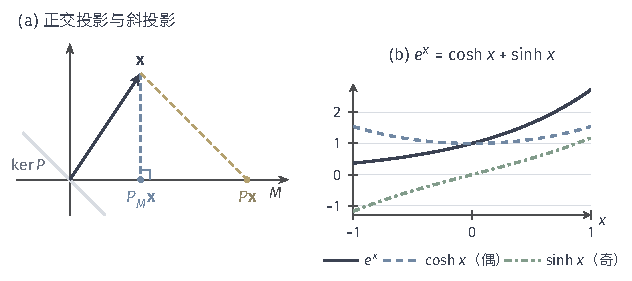
\includegraphics[width=107.0mm]{figures/02-abstract-mathematics/03-function-spaces/tikz/c2-projections/figure.pdf}
  \caption{正交投影与斜投影、偶部分与奇部分。(a)~平面中$\bm x=(0.6,0.9)$到横轴$M$的正交投影为$(0.6,0)$（蓝），残差与$M$垂直；斜投影$P(x_1,x_2)=(x_1+x_2,0)$沿核$x_1+x_2=0$（灰线）把$\bm x$送到$(1.5,0)$（黄），残差不与$M$垂直；(b)~$L^2(-1,1)$中$e^x$分解为偶部分$\cosh x$（蓝虚线）与奇部分$\sinh x$（绿点划线），两部分正交。}
  \label{fig:lfo-projections}
\end{figure}

\paragraph{偶函数投影}
在$L^2(-1,1)$上令
\[
 (Pu)(x)=\frac{u(x)+u(-x)}{2}.
\]
直接验证$P^2=P$。自伴性来自变量替换$x\mapsto-x$保持Lebesgue测度：$\int_{-1}^1\overline{v(x)}u(-x)\,dx=\int_{-1}^1\overline{v(-x)}u(x)\,dx$，于是$\langle v,Pu\rangle=\langle Pv,u\rangle$。由定理~\ref{thm:lfo-orthogonal-projection}，$P$是正交投影，像是偶函数子空间，核是奇函数子空间，两者正交。

以$u(x)=e^x$为例，$Pu=\cosh x$，$(I-P)u=\sinh x$，如图~\ref{fig:lfo-projections}(b)。正交性可以直接核对：$\cosh x\sinh x$是奇函数，在$[-1,1]$上积分为零。勾股恒等式也可以复算：
\[
 \begin{aligned}
 &\|e^x\|^2=\int_{-1}^1e^{2x}\,dx=\sinh2\approx3.627,\\
 &\|\cosh x\|^2=1+\tfrac12\sinh2\approx2.813,\qquad
 \|\sinh x\|^2=\tfrac12\sinh2-1\approx0.813 ,
 \end{aligned}
\]
后两者之和正是前者。若把区间换成不对称的$[-1,2]$，或把测度换成不对称的权重，替换$x\mapsto-x$不再保持内积，同一公式就不再给出正交投影。

\paragraph{有限群平均（补充）}
偶函数投影是对二元群$\{x,-x\}$求平均。一般地，设有限群$G$由保持测度的可逆变换组成，令$(Pu)(x)=|G|^{-1}\sum_{g\in G}u(g(x))$。同样的变量替换说明$P$自伴，群的结构说明$P^2=P$，所以$P$是到$G$不变函数子空间的正交投影。这只是一个空间分解的事实；把数据或模型投影到不变子空间是否改善某个统计任务，需要另外的分析，不能由投影性质直接推出。

\subsection{条件期望的投影解释}
\label{sec:lfo-conditional-expectation}

正交投影最重要的概率实例是条件期望。本小节只补充它的空间解释，所用的条件期望定义与性质先就地写明。

\paragraph{所用的定义与性质}
设$(\Omega,\mathcal F,\mathbb P)$是概率空间，$\mathcal G\subset\mathcal F$是子$\sigma$代数。为避免与空间记号$X$冲突，本小节用$Z$表示随机变量，并只考虑实值情形。对可积的$Z$，\term{条件期望}（conditional expectation）$\mathbb E[Z\mid\mathcal G]$是满足
\begin{equation}
 \mathbb E\bigl[\mathbb E[Z\mid\mathcal G]\,\mathbf 1_A\bigr]=\mathbb E[Z\mathbf 1_A]\qquad(A\in\mathcal G)
 \label{eq:lfo-conditional-expectation}
\end{equation}
的$\mathcal G$可测可积函数，在几乎处处相等的意义下唯一。它的存在性由Radon--Nikodym定理给出，具体做法是取$\mathcal G$上测度$G\mapsto\int_G Z\,d\mathbb P$关于$\mathbb P|_{\mathcal G}$的密度。下面还要用到两个标准性质：条件期望是线性的；条件Jensen不等式给出$(\mathbb E[Z\mid\mathcal G])^2\leq\mathbb E[Z^2\mid\mathcal G]$几乎处处成立。这些性质的系统建立属于第~\ref{part:probability-spaces}部分；离散与有密度情形下的初等版本可参考\BookChapterRef{chap:random-vectors}{卷一“随机向量与联合分布”章}。

\paragraph{$\mathcal G$可测元素组成闭子空间}
令$L^2(\mathcal G)$为$L^2(\Omega,\mathcal F,\mathbb P)$中有$\mathcal G$可测代表的等价类全体，它是线性子空间。它是闭的：设$Z_n\in L^2(\mathcal G)$且$Z_n\to Z$于$L^2$，取各$Z_n$的$\mathcal G$可测代表；由第~\ref{sec:fs-convergence-modes}节，可抽子列$Z_{n_k}\to Z$几乎处处。令$W=\limsup_kZ_{n_k}$（在其取有限值处，其余处取零），它作为$\mathcal G$可测函数的上极限是$\mathcal G$可测的，并且几乎处处等于$Z$，所以$Z\in L^2(\mathcal G)$。这里取上极限而不是直接修改零测集，是为了避免例外零测集本身不属于$\mathcal G$。

\paragraph{条件期望在这个子空间中}
设$Z\in L^2$，记$W=\mathbb E[Z\mid\mathcal G]$。由条件Jensen不等式并对式~\eqref{eq:lfo-conditional-expectation}取$A=\Omega$的形式，
\[
 \mathbb E[W^2]\leq\mathbb E\bigl[\mathbb E[Z^2\mid\mathcal G]\bigr]=\mathbb E[Z^2]<\infty ,
\]
所以$W\in L^2(\mathcal G)$，并且$\|W\|_2\leq\|Z\|_2$。

\paragraph{误差与子空间正交}
接下来验证$Z-W$与$L^2(\mathcal G)$中的每个元素正交。式~\eqref{eq:lfo-conditional-expectation}说明对示性函数$V=\mathbf 1_A$（$A\in\mathcal G$）有$\mathbb E[(Z-W)V]=0$；由线性，对$\mathcal G$可测的简单函数也成立；有界$\mathcal G$可测函数是这类简单函数的一致极限，而$Z-W$可积，所以由控制收敛定理推广到有界的$V$。最后，对一般的$V\in L^2(\mathcal G)$，令截断$V_k=V\mathbf 1_{\{|V|\leq k\}}$，它有界且$\mathcal G$可测；由控制收敛定理$\|V_k-V\|_2\to0$，而内积连续，所以
\[
 \mathbb E[(Z-W)V]=\lim_k\mathbb E[(Z-W)V_k]=0 .
\]

\begin{theorem}[条件期望是正交投影]
\label{thm:lfo-conditional-expectation-projection}
设$Z\in L^2(\Omega,\mathcal F,\mathbb P)$。则$\mathbb E[Z\mid\mathcal G]$是$Z$在闭子空间$L^2(\mathcal G)$上的正交投影。因此$Z\mapsto\mathbb E[Z\mid\mathcal G]$是$L^2$上范数为$1$的自伴正算子，并且
\[
 \mathbb E[(Z-\mathbb E[Z\mid\mathcal G])^2]=\min_{V\in L^2(\mathcal G)}\mathbb E[(Z-V)^2] .
\]
\end{theorem}

\begin{proof}
前面已经说明$W=\mathbb E[Z\mid\mathcal G]\in L^2(\mathcal G)$且$Z-W\perp L^2(\mathcal G)$。由第~\ref{sec:fs-projection}节，满足这两个条件的元素唯一，就是正交投影，并且它是子空间中离$Z$最近的元素。由定理~\ref{thm:lfo-orthogonal-projection}，它是自伴正算子；常数属于$L^2(\mathcal G)$且被保持不变，所以范数等于$1$。
\end{proof}

\paragraph{均方误差的分解}
由第~\ref{sec:fs-projection}节的勾股恒等式，
\[
 \mathbb E[Z^2]=\mathbb E\bigl[(\mathbb E[Z\mid\mathcal G])^2\bigr]+\mathbb E\bigl[(Z-\mathbb E[Z\mid\mathcal G])^2\bigr].
\]
第一项是只用$\mathcal G$中的信息能解释的部分，第二项是这些信息解释不了的残差。定理中的极小性说明，在一切只依赖$\mathcal G$信息的平方可积预测中，条件期望的均方误差最小。

\paragraph{嵌套信息与塔式性质}
若$\mathcal G_1\subset\mathcal G_2$，则$L^2(\mathcal G_1)\subset L^2(\mathcal G_2)$。记$P_1,P_2$为相应的投影，先投影到大的子空间、再投影到小的子空间，等于直接投影到小的子空间：$P_1P_2=P_1$；而小子空间中的元素在大子空间上的投影是它自己：$P_2P_1=P_1$。翻译成条件期望，就是塔式性质
\[
 \mathbb E\bigl[\mathbb E[Z\mid\mathcal G_2]\bigm|\mathcal G_1\bigr]=\mathbb E[Z\mid\mathcal G_1]=\mathbb E\bigl[\mathbb E[Z\mid\mathcal G_1]\bigm|\mathcal G_2\bigr].
\]
$P_1P_2=P_1$的验证只需一行：$P_2Z-Z\perp L^2(\mathcal G_2)\supset L^2(\mathcal G_1)$，所以$P_1(P_2Z)-P_1Z=P_1(P_2Z-Z)=0$。

\paragraph{分块平均的例子}
取$\Omega=[0,1)$，$\mathbb P$为均匀分布，$Z(\omega)=\omega^2$。设$\mathcal G_4$由四个区间$[k/4,(k+1)/4)$生成，$\mathcal G_2$由两半生成。对有限个区间生成的$\sigma$代数，$\mathcal G$可测函数就是在各区间上取常数的函数，式~\eqref{eq:lfo-conditional-expectation}要求条件期望在每个区间上等于$Z$的平均值：
\[
 \mathbb E[Z\mid\mathcal G_4]=4\int_{k/4}^{(k+1)/4}\omega^2\,d\omega=\frac{(k+1)^3-k^3}{48},
\]
即依次为$1/48,7/48,19/48,37/48$；而$\mathbb E[Z\mid\mathcal G_2]$在两半上分别为$1/12$与$7/12$。图~\ref{fig:lfo-conditional-expectation}画出了这两个阶梯函数。粗分块的值正是细分块的值两两再平均，例如$(1/48+7/48)/2=1/12$，这就是塔式性质。

\begin{figure}[!htb]
  \centering
  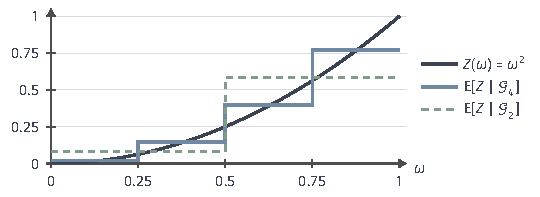
\includegraphics[width=91.4mm]{figures/02-abstract-mathematics/03-function-spaces/tikz/c2-conditional-expectation/figure.pdf}
  \caption{条件期望作为分块平均。$\Omega=[0,1)$上的均匀概率，$Z(\omega)=\omega^2$（黑）。$\mathcal G_4$由四个等长区间生成，$\mathbb E[Z\mid\mathcal G_4]$（蓝）在各区间上取$Z$的平均值$1/48,7/48,19/48,37/48$；$\mathcal G_2$由两半生成，$\mathbb E[Z\mid\mathcal G_2]$（绿虚线）取$1/12,7/12$，恰为细分块值的两两平均。}
  \label{fig:lfo-conditional-expectation}
\end{figure}

均方误差分解也可以复算。$\mathbb E[Z^2]=\int_0^1\omega^4\,d\omega=1/5$。四块时，$\mathbb E[W_4^2]=\frac14\cdot\frac{1+49+361+1369}{48^2}=\frac{1780}{9216}\approx0.1931$，残差约为$0.2-0.1931=0.0069$；两块时，$\mathbb E[W_2^2]=\frac12(\frac1{144}+\frac{49}{144})\approx0.1736$，残差约为$0.0264$。信息越细，子空间越大，投影离$Z$越近。两次投影之间的差$W_4-W_2$与$W_2$正交，$\mathbb E[(W_4-W_2)^2]=\frac{180}{9216}\approx0.0195$，恰好补足$0.1931-0.1736$。

本小节补充的是空间解释，没有重新建立条件期望的存在性。鞅、滤波与状态估计等以条件期望为基础的随机过程问题，可参考\BookChapterRef{chap:random-sequences-and-processes}{卷三“随机序列与随机过程”章}。
